\chapter{Implementation}
In this chapter we describe in details the framework that we implemented for testing the SQL-compliance for current DBMSs.


\section{Implementation}
The framework is composed by different tools such as random SQL generator engine, comparison tool and random data generator.  All tools are implemented in Java programming language which can run on all platforms that support Java except the random data generator which we use an open source python script that can generate realistic datasets.

 \begin{figure} 
      \centering
      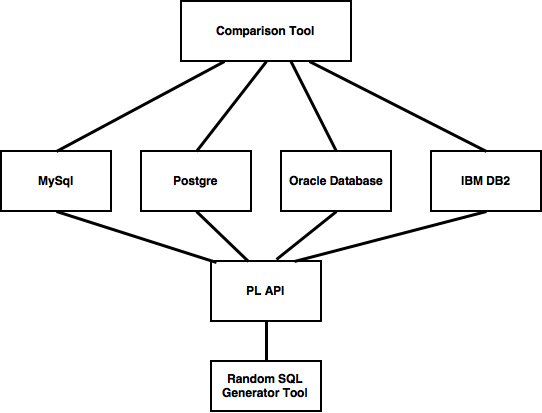
\includegraphics[width=\textwidth]{Images/Chapter4/1-implemen_detail}
      \caption{Random SQL Generator Architecture}
      \label{fig:counting-methods}
    \end{figure}


\subsubsection{Random SQL generator engine}
One of the most important components of the framework is the random SQL generator tool which can be used to generate thousand of different queries for evaluating the current DBMSs. Obviously SQL language has a strong power expressivity and as a consequence it supports many commands where some of them are simple in terms of their use such as SELECT, FROM, WHERE and some other more trickier such as GROUP BY, HAVING or aggregation functions where we need to care about the proper use of these commands and generating syntactically correct SQL queries. As a result, for achieving that our implementation is composed by various classes where each of them is used for different purpose. It is worthy mentioning that the tool can be used by its own use for other purposes. Thus, in this work, we have designed and implemented this tool from scratch using Java programming language. In addition, the tool has been designed in a way that it is modular and reusable for supporting new DBMSs in the future without the need of changing the whole structure of the tool. Thus, the main idea of the tool is to generate a diversity of queries for testing the DBMSs.  
The random SQL generator tool is consisted by different Java classes and a configuration file. An important consideration was how to design our generator tool in a way that will be feasible to generate different valid SQL queries and at the same time to be syntactically correct. Hence, we have implemented an internal representation for generating randomly SQL queries and each class is responsible for generating a different statement  that contribute to the overall query. For example, one of the classes that constitutes the tool is the SELECT class which obviously this class is responsible for generating the SELECT clause of each SQL query. Having different classes for each clause, it makes it easier to extend the tool in order to add new functionality and at the same time there is no need to change other part of the code. The final SQL query is converted to an SQL string and is executed to the current DBMSs. It is not feasible to generate SQL strings directly because we need to track things. If we generating just strings, it will not possible to check if in the WHERE clause it is mentioning attributes that appear in the FROM clause or they comes as parameters from the outer query. Thus, there is a need to track attributes for each clause. 
Another important consideration that we had to think about was how to avoid generating completely random SQL queries. Even though we need to generate random SQL queries to stress the existing DBMSs in different situations, we need to control some characteristics of the SQL query. For example, imagine an SQL query that performs a cartesian product with a large number of tables. In this situation, we will have as a consequence the query to be executed for a long time or even for ever and it is not so useful for our goal. Many parameters can be specified from the configuration file such as maximum level of nesting, max number of tables in a FROM, probability of having arithmetic comparisons. More details about the configuration file is given subsequently. As a consequence, our tool supports a configuration file that can be used to control the randomly generated SQL queries. Below is provided a part of the configuration file and some of the main parameters are explained.     

It can be seen from the configuration file that we can control many parameters, nevertheless it does not imply that we restrict the diversity of SQL query that can be generated. For example, we can set an upper bound of tables that appear in the FROM clause. In that way, we avoid having an enormous table size from cartesian product. In addition, even it is not so usual to have constant comparison in an SQL query, nevertheless SQL standards support this. Thus, we generate SQL queries which have constant comparisons but we do not need to have a lot of such queries. An example of such query is as follow:

SELECT r41.A AS A0
FROM r4 AS r41
WHERE 1 > 2

We can specify the probability of having such cases by setting the parameter probWhrConst which have a domain between 0 and 1 meaning that if the value is 1 then there will be exist for sure a constant comparison.
	Another important parameter which can be specified from the configuration file is the level of nesting. We can randomly generate SQL queries with a specific level of nesting. The example below demonstrates a query with level of nesting three. For generating such a query many consideration should be taken into account. For example, we should track attributes for outer queries, as inner query can access outer attributes or attributes from its FROM clause. The opposite is not true, meaning that we cannot access attributes from an inner query. 





SELECT r12.A AS A0, r12.B AS A1, r22.A AS A2 
FROM r1 AS r12, r2 AS r22
WHERE NOT(NULL <> 9 OR r12.A >= r22.A OR ( NOT(5 > 3 )  ) 
AND r12.A = ANY( (	SELECT r43.B AS A0
			FROM r4 AS r43, r1 AS r13, r2 AS r23
			WHERE (NULL >= 3)AND r22.B IN (SELECT r43.A AS A0
							FROM r4 AS r44, r2 AS r24
							WHERE (15 < 2 AND NOT(NULL >= 14 ) ) 



	Another important decision that should be taken into account is how we can provide the relations and attributes to the tool. An initial approach was to be given as parameters in the configuration file. Albeit this approach works pretty well, it makes our tool not portable. Image if the DBMSs have lots of tables with many columns. Hence, It will be time-consuming to give these parameters via the configuration files. Thus, an efficient approach is to retrieve the whole schema from DBMSs automatically. As a result, our tool has the capability to automatically retrieve the whole schema for any DBMS just by providing the credential for connecting to the database in the configuration file.

\section{Comparison Tool} 
As it was mentioned the purpose of the random query generator tool is to generate thousand of SQL queries which can be then used to evaluate current DBMSs. The result of each query can be huge in terms of its cardinality with different order. As a consequence, there was a need to automate the process and identify any difference that may exist by comparing the results efficiently. Therefore, we illustrate below our comparison tool (CT) which has been implemented for achieving the aforementioned goal and further we provide a detailed explanation about the internal implementation of the tool.  

 \begin{figure} 
      \centering
      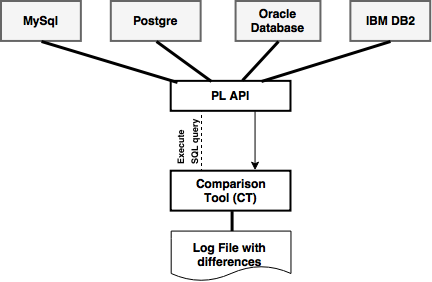
\includegraphics[width=\textwidth]{Images/Chapter4/2-ComparisonTool}
      \caption{Simple Architecture of Comparison Tool}
      \label{fig:counting-methods}
  \end{figure}

We have implemented the CT in Java programming language in order to compare the output results of each DBMSs. The tool is an important component of our project as it is used to conduct our experiments and identify the main differences that exist between current DBMSs. Apparently, differences may be minor or extremely difficult to be identified as DBMSs try to follow the SQL standards. Nevertheless, we illustrate in our experiments that differences exist and in some of the cases may be significant depends on the context that DBMSs are used. Comparing the results of each SQL query is not an easy task because each DBMSs use different algorithms to evaluate them and they return the output results in different order or their output format differ. The CT is fully compatible with the random generator engine and it takes as input each SQL query which is generated by the random SQL generator and subsequently evaluates each query to the current DBMSs. As a result, we use a data structure, namely LinkedList to store each row and then we use an efficient in-memory sorting algorithm to sort the rows. Then, we compare each rows of each DBMS and check if any row differ or does not exist. In case where the results are not identical, a log file is generated and we record which DBMSs differ and what is the SQL query that cause the problem.

 \begin{figure} 
      \centering
      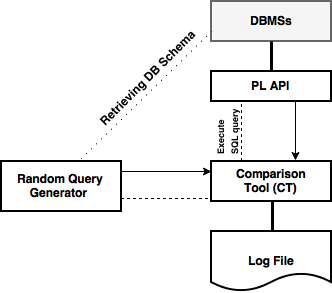
\includegraphics[width=\textwidth]{Images/Chapter4/3-ComparisonTool}
      \caption{Architecture of Comparison Tool}
      \label{fig:counting-methods}
  \end{figure}


\section{Generate data}
Datafiller is a well-known open-source project that provides the capability of generating random data. Thus it will be used in this project for generating a diversity of  data sets in order to evaluate all major DBMSs. More precisely, the datafiller script generates random data, based on a data schema which is given as a parameter, and by taking into account constraints of that schema. For example, it takes into account the domain of each field and if the field should be unique, foreign key or primary key. Another important parameter is the df: null=x.xx% which indicated nullable rates. It will be extremely useful to test the behaviour of current DBMS in a database with nulls and check if there are differences.     

Additionally, more complex parameters can be provided as well, such as a number of tuples per table using --size SIZE parameter. It worthy mentioning that these parameters should be defined within the schema script and should start with -- df.  Further, we can generate more realistic data by providing some information in the schema script of the database. For example, if we have a field that represents a date, then we can provide a specific range in order for the datafiller to generate dates only within this range. This can be achieved by specifying the following parameter: range -- df: start=year-month-day end=year-month-day beside the date field. Subsequently, we need to add the --filter parameter while running the script. These are only some of the important parameters that the datafiller provides but apart from these, it provides more sophisticated properties which are out of importance for our project.

It is important mentioning that the datafiller does not support importing data to other databases such as Oracle database, MS Server or IBM DB2 except postgresSQL. As a result, our approach is to import the data in postgreSQL and then export the random generated data in a CSV files. In this way, we can import the CSV files in all the DBMS, as all of them support importing data from CSV files.  

